\chapter{Fundamentals}
\label{chap:fundamentals}

Under the term \emph{ray tracing} we understand the utilization of algorithms that involve the casting of virtual light rays for generating images. The purpose of these light rays is to archive high visual realism by the simulation of natural behavior in real life. 

The reason we are able to perceive nearby objects or persons is due to the fact that light, which is being emitted from light sources, either natural or artificial, is interacting with these objects or persons. It is being reflected off their surfaces towards our vision sensory organs after possibly being reflected a multiple times before from other surfaces.

The purpose of ray tracing algorithms is to imitate this behavior, usually by tracing these light rays in reverse order from the sensory organs (or a virtual camera or an "eye point") back to the emitting light source.

\begin{figure}[h]
	\centering
	\includegraphics[width=.9\linewidth]{img/1 fundamentals/ray_tracing.png}
	\caption{Ray tracing procedure for calculating global illuminate.}
	\label{fig:raytracer_general}
\end{figure}

An advantage of these ray tracing algorithms is that the core procedure is straightforward when viewed from a theoretical point of view. Figure \ref{fig:raytracer_general} shows an example of a virtual scene. It is composed of an orange sphere, a white ground plane, and a light source. Furthermore, there exists an image plane on which the 2D image of the 3D scene will be projected. A ray is consisting of two components, an origin point and a direction vector. The "Eye Point" in \ref{fig:raytracer_general} will serve as the origin of the cast rays (sometimes, the Eye Point is referred to as camera or virtual camera). In the figure, the image plane is composed of multiple quadratic "cells" that represent the actual pixels of the resulting image. Through each of these cells, a ray is cast into the scene from the eye point. The subsequent step is to determine, whether that ray hit a particular geometry by performing intersection tests on all geometries in the scene \footnote{Testing all geometries present in a complex scene for intersection is a naive approach and not practical. Section \ref{sec:acceleration} introduces some common ray acceleration data structures to compensate for this.}. In case a geometry is hit, a secondary ray is generated with its origin at the intersection point and its direction toward the light source. In case this secondary light ray does not intersect any other geometry between its origin and the light source, this means that the first intersection point is exposed to light and the material color at that point is used for the corresponding pixel (see R1 in figure \ref{fig:raytracer_general}). Otherwise, the intersection point must be in shadow (see R2). This procedure generates an image with local illumination.

The following chapter is dedicated to providing background information on ray tracing, shape representation in rendering systems, and ray acceleration data structures. Furthermore, the Embree framework is introduced.

\section{Ray Tracing Algorithms}

The following section outlines the development of various ray tracing techniques. The pioneering work of \cite{appel1968some} and \cite{whitted1979improved} will be discussed, and the derivation to the rendering equation \cite{kajiya1986rendering}, whose solving via Monte Carlo integration is the aim of modern rendering environments, will be presented.

\subsection{Origins of Ray Tracing}
As briefly mentioned in the Introduction, ray tracing was pioneered in 1968 by \cite{appel1968some}. The aim of his work was to provide basic shading for wire framed solids, yielding a better communication of spatial relation and depth of objects in the rendered image.

In order to achieve this shading, virtual light rays are shot from a scene light source in random directions. Whenever one such ray intersects a geometry, a character or symbol (e.g. a small "plus"-symbol or square) is placed at that intersection point. If enough such rays would be cast, areas on the solid that are exposed to light would be shaded by these symbols.
The result would then come to be by inverting the shaded and non-shaded areas of the geometry.

The intensity of light $I$ incident to the light source is described by the following equation:

\begin{equation}
I = S\frac{\cos{\theta}}{{D}^2}
\end{equation}

\noindent where
\begin{itemize}
	\setlength\itemsep{0.05em}
	\item  $S$ is the intensity of the light source,
	\item  $\cos\theta$ is the angle between the ray and the surface normal at the intersection point, and
	\item  $D$ is the distance between intersection point and light source.
\end{itemize}

\begin{figure}[h]
	\centering
	\includegraphics[width=1\linewidth]{img/1 fundamentals/appel_comp}
	\caption{Original figures from \cite{appel1968some}. The left figure shows plain solid geometry and the right figure shows the same solid with shading applied to it.}
	\label{fig:appel}
\end{figure}

Figure \ref{fig:appel} shows the result. Without the additional shading information, it would be difficult for the observer to perceive the position of the upper geometry relative to the plane.

In order to achieve convincing results, a high number of rays had to be generated ("Even for about 1000 light rays results were splotchy." \cite[p 3]{appel1968some}). At the time of publication, computational power of hardware could hardly be used for this approach.

The idea of casting rays later became a key utilization for a shading model that aimed for higher realism by taking the "global setting" of geometries into account \cite{whitted1979improved}. A variety of shading models existed at that time, which were able to convincingly display optical effects. However, these models usually worked only in special cases and not well with each other, as noted by Andrew Glassner in the preface of his book \citetitle{glassner1989introduction} \cite{glassner1989introduction}. Some models existed that were good at calculating reflection effects, but could not handle refraction effects well. And vice versa. 

\cite{whitted1979improved} introduced a shading model that would truthfully simulate reflection, shadows and refraction as well as the effects of other conventional shading models at that time.  

The model is partially derived from an empirical reflection model developed by \cite{phong1975illumination}, which assumes that light, which is reflected from a surface, is composed by three types of reflection: ambient reflection, diffuse reflection and specular reflection. The following equation describes this model:

\begin{equation} \label{eq:phong}
I = k_{a} + k_{d}\sum_{j}(n*L_{j}) + k_{s}\sum_{j}(n*L_{j}\prime)^{\alpha}
\end{equation}

\noindent where
\begin{itemize}
	\setlength\itemsep{0.05em}
	\item  $I$ is the reflected intensity,
	\item  $I_{a}$ is the ambient reflection coefficient,
	\item  $k_{d}$ is the diffuse reflection coefficient,
	\item  $k_{s}$ is the specular reflection coefficient,
	\item  $n$ is the unit surface normal at an intersection point,
	\item  $L_{j}$ is a vector in the direction of the $j$th light source,
	\item  $L_{j}\prime$ is a half vector between the eye point and the $j$th light source, and
	\item  $\alpha$ is the glossiness coefficient.
\end{itemize}

This model even nowadays finds popularity among real time graphics due to its low computational cost and convincing (although not physically plausible) results.
The model assumes furthermore that light sources are located at an infinite distance from the scene geometry, and thus, it does not account for objects within the scene acting as light sources. It was noted in \cite{newell1977progression}, that this assumption can critically affect the specular reflection component of Equation \ref{eq:phong}.

\begin{figure}[h]
	\centering
	\includegraphics[width=.7\linewidth]{img/1 fundamentals/whitted.png}
	\caption{Light intensity propagated towards an observer being composed of a specular reflection component $S$ and a transmissive reflection component $T$.}
	\label{fig:whitted_model}
\end{figure}

As opposed to the Phong shading model, Whitted's model assumes that the light intensity $I$ arriving at the $Eye Point$ from the intersection point $x$ along the outgoing direction $\omega_{o}$ is conglomerated by a specular reflection component $S$, being propagated along direction $\omega_{s}$ and a transmission component $T$, being propagated along direction $\omega_{t}$. This is shown in Figure \ref{fig:whitted_model}.
The model is given by the equation:
\begin{equation} \label{eq:whitted}
I = k_{a} + k_{d}\sum_{j}(n*L_{j}) + k_{s}S + k_{t}T
\end{equation}

\noindent where
\begin{itemize}
	\setlength\itemsep{0.05em}
	\item  $S$ is the light intensity of the specular reflection
	\item  $T$ is the light intensity of the transmission, and
	\item  $k_{s}$ is the transmission coefficient
\end{itemize}
The ambient and diffuse term are maintained from Equation \ref{eq:phong}. 

The model is capable of generating images with a high degree of realism, preconditioned that the coefficients of equation \ref{eq:whitted} are reasonably chosen. Whitted noted in his paper that "for the best
accuracy they [the coefficients] should be functions that incorporate an
approximation of the Fresnel reflection". 
Generally, Equation \ref{eq:whitted} approximates the reflection of light towards an observer (or camera, or "Eye Point") from a single surface. However, in nature, light that is propagated towards a viewer from a surface most certainly has interacted with other surfaces before. If true realism of computer generated images is desired, these previous interactions have to be taken into consideration, even for virtual scenes with moderately complex geometry. An example of such an event can be seen in Figure \ref{fig:whitted_rays}.

\begin{figure}[h]
	\centering
	\subfloat[Light is being reflected from other surfaces before reaching the Eye Point.]{\includegraphics[width=.6\textwidth]{img/1 fundamentals/whitted_rays.png}\label{fig:whitted_rays}}
	\hfill
	\subfloat[Tree structure storing the individual reflection and transmission components.]{\includegraphics[width=.3\textwidth]{img/1 fundamentals/whitted_tree.png}\label{fig:whitted_tree}}
	\caption{Figures based on the original figures from the paper \citetitle{whitted1979improved} \cite{whitted1979improved}}
\end{figure}

This natural behavior is implemented in the following way. From the $Eye Point$, a ray is cast towards the virtual scene and a possible intersection point $x$ with the scene geometry is calculated. 
The transmission and specular component rays at that intersection point are then recursively calculated by Equation \ref{eq:whitted} and stored in a tree structure which is shown in Figure \ref{fig:whitted_tree}. 
Each node in this tree represents an intersection point and is furthermore associated with rays pointing towards each light source in the scene, which are correlated to the $L_{j}$ terms in Equation \ref{eq:whitted}. If one of these light rays $L_{j}$ intersect scene geometry before it reaches light source $j$, the intersection point corresponding to the tree node in question is not illuminated by that particular light source and consequentially the contribution of it to the reflection is not taken into consideration. To prevent a branch of the tree from growing infinitely large, it is truncated as soon as an attempt is made to access more storage than was previously made available for it. After such a tree is created, it is traversed recursively in order to calculate the light intensity at each node with Equation \ref{eq:whitted}, finally resulting in the calculation of the total light intensity that is reflected towards the $Eye Point$. Between two nodes, the intensity is attenuated according to a distance function between the intersection points, associated with the node and the node's parent node. 
Such trees are created and traversed for every pixel of the image plane. This procedure allows for the convincing display of a variety of optical effects with the help of a single model.

\subsection{The Rendering Equation}

In 1986, an integral equation was developed by Kajiya \cite{kajiya1986rendering}, that would describe the total reflected radiance towards an observer as the "sum" (or integral) of all light contributions over a hemisphere at a point on the surface. This mathematical model achieves high realism by taking direct illumination (light from light sources) and indirect illumination (light being reflected off other surfaces in the scene) into account.
The so-called \emph{rendering equation} is given by

\begin{equation}\label{eq:renderingeq}
L(x, \omega_{o}) = L_{e}(x, \omega_{o}) \int_{H(x)} L(x, \omega_{i})f_{r}(\omega_{i} \rightarrow \omega_{o})\cos\theta\partial\omega_{i}
\end{equation}

\noindent where
\begin{itemize}
	\setlength\itemsep{0.05em}
	\item  $L(x, \omega_{o})$ is the total reflected light intensity from a surface point $x$ towards the observer along the outgoing direction $\omega_{o}$,
	\item  $L_{e}(\omega_{o})$ is the radiance emitted at the surface point $x$ and propagated along $\omega_{o}$,
	\item  $H(x)$ is the hemisphere over surface point $x$,
	\item 	$L(x, \omega_{i})$ is the light intensity incident to $x$ along direction$\omega_{i}$, 
	\item  $f_{r}(\omega_{i} \rightarrow \omega_{o})$ is the bidirectional reflectance distribution function (BRDF), and 
	\item  $\cos\theta$ is a term, compensating for Lambert's cosine law.
\end{itemize}

For a better understanding of the individual terms of the rendering equation, a definition of radiance and a brief explanation of the \emph{bidirectional reflectance distribution function} and the local reflection equation is provided in the following subsections.
The information provided by these subsections are collated from the lecture notes of the course \citetitle{cg3} held at Charles University in Prague, Czech Republic \cite{cg3}, from the book \citetitle{pharr2016physically} \cite{pharr2016physically} and from the book \citetitle{hughesDamEtAl13} \cite{hughesDamEtAl13}.

\subsubsection{Definition of Radiance}

We define the \emph{radiance} of a source, sometimes informally referred to as "brightness", as the power per unit area $\partial A$ perpendicular to the ray in the direction $\omega_{o}$ and per unit solid angle that is propagated along it (see Figure \ref{fig:radiance}). This is described by the following equation:

\begin{equation}
L(\omega_{o}) = \frac{\partial^2\phi}{\partial\omega_{o}\partial A\cos\theta}
\end{equation}

\noindent where
\begin{itemize}
	\setlength\itemsep{0.05em}
	\item  $\omega_{o}$ is the outgoing direction
	\item  $\phi$ is flux or radiance per unit time
	\item  $A$ is the surface area, and
	\item  $\cos\theta$ a term for compensating Lambert's cosine law
\end{itemize}

\begin{figure}[h]
	\centering
	\subfloat[Radiance is defined as the radiant flux emitted, received or reflected per solid angle $\partial\omega_{o}$ per unit projected area $\partial A$.]{\includegraphics[width=.4\textwidth]{img/1 fundamentals/radiance.png}\label{fig:radiance}}
	\hfill
	\subfloat[The BRDF is a function defining how much light from the incoming direction$\omega_{i}$ is reflected towards the viewer along the outgoing direction $\omega_{o}$.]{\includegraphics[width=.5\textwidth]{img/1 fundamentals/brdf.png}\label{fig:brdf}}
	\caption{Diagrams visualizing radiance (Figure \ref{fig:radiance}) and the BRDF (Figure \ref{fig:brdf}).}
\end{figure}

From this definition we can derive the bidirectional reflectance distribution function.

\subsubsection{Bidirectional Reflectance Distrubution Function (BRDF)}
The bidirectional reflectance distribution function (BRDF) is a mathematical model describing the reflection properties of a given surface. To be precise, it describes the probability of light energy, arriving at a point $x$ on a surface from direction $\omega_{i}$, being reflected along the reflection $\omega_{o}$. 
The BRDF model is defined by:

\begin{equation} \label{eq:brdf}
f_{r}(\omega_{i} \rightarrow \omega_{o}) = \frac{\partial L_{r}(\omega_{o})}{L_{i}(\omega_{i})\cos\theta\partial\omega_{i}}
\end{equation}

\noindent where
\begin{itemize}
	\setlength\itemsep{0.05em}
	\item  $L_{r}(\omega_{o})$ is the reflected light energy, and
	\item  $L_{i}(\omega_{i})$ is the incident light energy
\end{itemize}

Properties of BRDFs are the conservation of energy and the Helmholtz reciprocity, stating that the incident light and reflected light in Equation \ref{eq:brdf} can be switched without affecting the result. There exist different types of BRDFs: empirical BRDFs, physically based BRDFs and BRDFs being an approximation of measured data.
BRDFs are a crucial component when calculating direct illumination with the \emph{local reflection equation}.

\subsubsection{Local Reflection Equation}

The local reflection equation describes how much total light is reflected towards a given direction $\omega_{o}$. It is given by:

\begin{equation}\label{eq:local}
L_{r}(x, \omega_{o}) = \int_{H(x)} L_{i}(x, \omega_{i})f_{r}(\omega_{i} \rightarrow \omega_{o})\cos\theta\partial\omega_{i}
\end{equation}

\noindent where
\begin{itemize}
	\setlength\itemsep{0.05em}
	\item  $H(x)$ is a hemisphere over the interaction point $x$.
\end{itemize}

The total amount of reflected energy is calculated by the integration of all contributions of incident radiance over the hemisphere $H(x)$. The BRDF serves as a weight in this equation because only the energy reflected along $\omega_{o}$ is considered.
Figure \ref{fig:cb_local} shows the Cornell Box, where for each pixel Equation \ref{eq:local} was evaluated. The appearance of the scene is the result of shooting a ray into the scene, calculating a possible intersection point and then generating a second ray in the direction of the light source. However, the appearance of the Cornell Box is not physically realistic because the ceiling is not illuminated. This is due to the fact that with this approach no light rays that interact with surface points on the ceiling can directly reach the missive area of the light source. And this is where the rendering equation comes into play. \todo{definetely rephrase}
 
\subsubsection{The Rendering Equation Revisited}

The rendering equation, which for reasons of convenience is shown again in Equation \ref{eq:renderingeq2} is an extension of the local reflection equation which additionally takes global illumination information into account. 

\begin{equation}\label{eq:renderingeq2}
L(x, \omega_{o}) = L_{e}(x, \omega_{o}) \int_{H(x)} L(x, \omega_{i})f_{r}(\omega_{i} \rightarrow \omega_{o})\cos\theta\partial\omega_{i}
\end{equation}

Essentially, it describes the total reflection of energy towards direction $\omega_{o}$ from a surface point $x$ as the "sum" or integral of all the light intensity, incident to all directions over a hemisphere over the point $x$, together with the intensity emitted from point $x$, if $x$ is located on an emissive material. The unknown variable $L$ is present on both sides of this equation.

This function is a higher order integral which is difficult to calculate. The most common approach on solving this equation is the approximation via Monte Carlo methods. Monte Carlo methods numerically approximate a given integral by drawing random samples. The convergence speed of this procedure is independent of the dimension of the integral. Most of today's image synthesis algorithms utilize Monte Carlo methods to numerically approximate the solution of the rendering equation.


\begin{figure}
	\centering
	\subfloat[]{\includegraphics[width=.4\textwidth]{img/1 fundamentals/cb_direct.png}\label{fig:cb_local}}
	\hfill
	\subfloat[]{\includegraphics[width=.4\textwidth]{img/1 fundamentals/cb_global.png}\label{fig:cb_global}}
	\caption{The Cornell Box scene with local illumination (Figure \ref{fig:cb_local}) and global illumination (Figure \ref{fig:cb_global}).}
\end{figure}



\subsubsection{Path Tracing}

Multiple approaches for solving the rendering equation exists, for example the \emph{radiosity} method \cite{goral1984modeling}, aiming at solving it via the application of the finite element method. However, the most commonly used methods for solving the rendering equation are Monte Carlo methods. One particular Monte Carlo method is \emph{path tracing}, which is the subject of this section.

\begin{figure}
	\centering
	\includegraphics[width=1\linewidth]{img/1 fundamentals/path_tracing.png}
	\caption{Tracing a path for calculating global illumination.}
	\label{fig:pathtracing}
\end{figure}

Path tracing generates "paths" of light rays, starting at the $Eye Point$ and ending at a light source. An example of such path is visualized in Figure \ref{fig:pathtracing}. At each intersection point along the path, the intersected geometries are tested for occlusion and, if the shape is not occluded by another geometry, the direct contribution of the light source(s) are accumulated. 
To prevent the calculations of unprofitable paths, a path is continued according to a so-called "survival probability". This probability can e.g. be formulated as the reflectivity of the surface which is intersected by a ray. If this surface for example reflects only ten percent of light energy, the path is continued with a probability of then percent.
To approximate the integral part of the rendering equation, numerous paths are generated at the intersection point $x$. To generate the final color of the image pixels, the results calculated by the paths are averaged.

\begin{figure}
	\centering
	\includegraphics[width=.7\linewidth]{img/1 fundamentals/rendering_eq_figure.png}
	\caption{Original figure from the paper \citetitle{kajiya1986rendering} by Kajiya \cite{kajiya1986rendering}.}
	\label{fig:kajiya_figure}
\end{figure}

With regard to path tracing, we can re-write the rendering equation shown in \ref{eq:renderingeq} in the following way:
\begin{equation}\label{eq:renderingeq_update}
L(x, \omega_{o}) = L_{e}(x, \omega_{o}) \int_{H(x)} L(ray(x, \omega_{i}), -\omega_{i})f_{r}(\omega_{i} \rightarrow \omega_{o})\cos\theta\partial\omega_{i}
\end{equation}

The function $ray(x, \omega_{i})$ recursively calculates the incoming radiance for all directions around the point $x$. A visual result of evaluating this function for each pixel in an image can be seen in Figure \ref{fig:cb_global}.

In comparison of the ray tracing method of \cite{whitted1979improved}, path tracing is capable of simulating advanced optical effects such as soft shadows and diffuse interreflection.

\section{Solid Representations in 3D Space}

A crucial part of ray tracing algorithms is the calculation of intersection points between rays with scene geometry.
The representation of solid objects in the Euclidean space varies, thus does testing them for intersections with given rays. The following section illustrates three types of solid representations in image synthesis environments, such as ART: Analytic surfaces, polygon meshes and constructive solid geometry.

\subsection{Analytical Surfaces}
\label{sec:quadrics}
Analytical surfaces are surfaces in three dimensional Euclidean space, defined by analytic functions. Common analytical surfaces are quadric shapes (or quadrics). Examples of this type of surface representation are spheres, cones, cylinders and paraboloids. The equations describing these shapes can be in implicit form, which has the pleasant property, that testing whether a point $p$ is located at the boundary of such a surface is easy. Generally speaking, implicit equations are relations of the form  $f(x_{0}, x_{1}, ..., x_{n}) = 0$ where $f$ is a function of multiple variables. Consider such a variable as a point $p$ in three dimensional space and evaluated by function $f$. An evaluation of $f$ will result in two possible outcomes: either $f(p) = 0$, which means $p$ is located on the surface of the shape, or  $f(p) \ne 0$, which means the opposite.
Due to this evaluation, quadrics are well suited for intersection testing during ray tracing.
In the following we will provide an example of an intersection calculation between a given unit sphere $S$ with radius $1$ and a given ray $R$. 

\begin{figure}[h]
	\centering
	\includegraphics[width=.5\linewidth]{img/1 fundamentals/sphere_isect.png}
	\caption{Intersection between a sphere $S$ with its center point $c$ and radius $r$, and a ray with origin $P$ and direction $\omega$. We attempt to solve a quadradic equation in oder to obtain points $t_{0}$ and $t_{1}$. For reasons of simplicity, visualized in two dimensional space.} 
	\label{fig:sphere_isect}
\end{figure}

The sphere $S$ is implicitly defined by: 
\begin{equation} \label{eq:sphere}
S(x,y,z) = x^{2}+y^{2}+z^{2}-1 = 0
\end{equation}
The ray $R$ in its parametric form is defined by:
\begin{equation}\label{eq:ray}
R(t) = P + t\omega
\end{equation}

\noindent where
\begin{itemize}
	\setlength\itemsep{0.05em}
	\item  $P$ is the origin of ray $R$, a point in Euclidean space,
	\item  $t$ a scalar, and
	\item  $\omega$ the direction vector of $R$.
\end{itemize}

To obtain the two intersection points, the parametric equation defining $R$ is substituted into the implicit equation defining $S$
\begin{equation}\label{eq:substitution}
(P_{x}+t\omega_{x})^{2}+(P_{y}+t\omega_{y})^{2}+(P_{z}+t\omega_{z})^{2}-1 = 0
\end{equation}
and then, since all variables with the exception of $t$ are known, solved for $t$.
Once the two resulting values $t_{0}$ and $t_{1}$ are obtained, the two intersection points $I_{0}$ and $I_{1}$ can be expressed as $I_{0} = P + t_{0}\omega$, and respectively $I_{1} = P + t_{1}\omega$.

\subsection{Polygon Meshes}

Polygon meshes represent shapes as a composition of multiple smaller polygons that are connected with each other via shared edges. The higher the number of such polygons the mesh exhibits, the higher the accuracy of the approximation of the represented shape. The most common types of polygons used are triangles and quadrangles. An example of a representation of a shape with a triangle mesh can be seen in Figure \ref{fig:poly_mesh}. These polygons are composed of a list of vertices, a list of edges connecting these vertices and a face, the area bounded by the vertices and edges. This information is sufficient to describe a polygon in 3D space. A reason why triangles are the most commonly used polygon for meshes is the efficient storage in memory and the property that the vertices of a triangle can never be not co-planar.

\begin{figure}
	\centering
	\includegraphics[width=.8\linewidth]{img/1 fundamentals/poly_mesh.png}
	\caption{Polygon mesh of the famous Utah Teapot, rendered with Blender \cite{blender2018}}
	\label{fig:poly_mesh}
\end{figure}

Various ray primitive intersection algorithms exist, for example the Möller– Trumbore intersection algorithm \cite{moller1997fast} for intersecting triangles. In order to test a given ray for intersection with a polygon mesh, theoretically all polygons contained in the mesh in question must be tested for intersection. This is of course a naive approach, since the number of intersection tests that need to be performed is linear in the number of polygons. As such polygon meshes are often composed of several thousand polygons, and testing them all for intersection has a decisive influence on the performance of the rendering process. Section \ref{sec:acceleration} introduces acceleration data structures, aiming at the minimization of those intersection tests.

\subsection{Constructive Solid Geometry (CSG)}

The idea behind constructive solid geometry (CSG) modeling is the application of boolean set operations to geometry primitives in order to create more complex geometries. The boolean set operators are union (logical \texttt{OR}), intersection (logical \texttt{AND}) and difference (denoted as \texttt{SUB}-operator). 
Primitives are usually quadric surfaces such as spheres, cones and cylinders, however, polygon meshes can be regarded as CSG primitives, too. Figure \ref{fig:csg} shows the application of each boolean operator to two sphere primitives. Multiple of such set operations can be hierarchically ordered with the help of a binary tree structure, called the CSG-tree.   

\begin{figure} 
	\centering
	\subfloat[Union of two spheres (\texttt{OR} operator).]{\includegraphics[width=.3\textwidth]{img/1 fundamentals/or.png}\label{fig:csg_or}}
	\hfill
	\subfloat[Intersection of two spheres (\texttt{AND} operator).]{\includegraphics[width=.3\textwidth]{img/1 fundamentals/and.png}\label{fig:csg_and}}
	\hfill
	\subfloat[Left sphere with the right sphere "subtracted" from it (\texttt{SUB} operator).]{\includegraphics[width=.3\textwidth]{img/1 fundamentals/sub.png}\label{fig:csg_sub}}
	\caption{Boolean operators Union (\ref{fig:csg_or}), Intersection (\ref{fig:csg_and}) and Difference (\ref{fig:csg_sub}) applied to two sphere objects.}
	\label{fig:csg}
\end{figure}

One example of such CSG tree is provided in Figure \ref{fig:csg_tree}. Its leafs are associated with the geometry primitives, the nodes with the set operations. Due to the possibility that two primitives can be translated, rotated or scaled before a boolean operator is applied to them, edges of the tree are associated with transformation information (this is denoted in the figure with the matrix icon). The transformation corresponding to an edge between a node and a node's parent can be "empty", meaning that it has no effect on the primitive represented by that node.  

\begin{figure}
	\centering
	\includegraphics[width=.9\linewidth]{img/1 fundamentals/csg_tree.png}
	\caption{Visualization of a CSG tree hierarchy, originally created by \cite{csgtree} and updated
	with a matrix icon symbolizing affine transformations of geometries.}
	\label{fig:csg_tree}
\end{figure}

\subsubsection{Ray Tracing with CSG}

The ray tracing of CSG was pioneered by \cite{roth1982ray}. In the algorithm, described in the paper \citetitle{roth1982ray}, the intersection calculation for a given ray during the ray tracing process is straightforward: 
All the primitives associated with the leaves of the CSG tree are tested for intersection. If an intersection test with a quadric shape for instance has a positive result, usually two intersection points are calculated: one point when the ray enters the primitive and one point when it exits it (there is the edge case that there exists infinitely many intersection points between a ray and a primitive when the ray is tangent to the primitive, however, this is seldom the case and can be safely ignored). \todo{fucking fix this sentence}Then the CSG tree is traversed bottom up, and each time an interior node, representing a boolean set operator, is encountered, the intersection points of the ray with the primitives associated with the child nodes are evaluated and re-arranged. For example, when considering the \texttt{OR} operator in Figure \ref{fig:csg_or}, and given that a single ray would intersect both spheres, there would be four intersection points: One entering the first sphere, followed by one entering the second sphere, then one exiting the first sphere, and finally one intersection point exiting the second sphere. The \texttt{OR} operator would treat the two spheres as one single object and therefore discard the interior intersection points. Similarly, the \texttt{AND} operator in Figure \ref{fig:csg_and} would discard the two intersections at the exterior of the spheres and keep the two intersections contained in both spheres.
And finally, the \texttt{SUB} operator in Figure \ref{fig:csg_sub} discards every intersection point on the sphere (exterior or interior) that is "subtracted" from the sphere on the left.
\todo{fucking fix this explanation}

The representation of CSG offers one significant advantage: Complex geometry can be expressed via the composition of a manageable amount of primitive shapes, as opposed to large numbers of polygons in a polygon mesh. Because testing whether a point lies inside or outside a primitive is easy, as noted in Section \ref{sec:quadrics}, and since the number of primitives of a composed CSG is usually lower than the amount of polygons in a polygon mesh, the number of intersection tests in each render pass is comparatively low.

Although the CSG modeling technique is several years old, it is still used in practice today, e.g. for computer-aided design.


\section{Spacial Acceleration Data Structures} \label{sec:acceleration}
The computational cost associated with ray tracing and path tracing algorithms has always been regarded as a "necessary evil" one has to face when desiring highly realistic images. An often cited fact is Whitted's observation, that, for complex scenes, 95 percent of the time used by his algorithm is spend on intersection calculations \cite[p 349]{whitted1979improved}. To give an example, the image displayed in Figure \ref{fig:kajiya_figure} was rendered via path tracing on an IBM 3081 machine during 1221 minutes \cite[p 149]{kajiya1986rendering}. The image had a resolution of 512 by 512 pixels and was rendered with 40 paths per pixel.

It was only a logical consequence, that over time, new ideas were introduced for accelerating the ray tracing process. Attempts can be the minimization of the number of rays that are cast into the scene, the development of faster intersection testing algorithms or the minimization of ray-primitive intersection tests. The upcoming of ray acceleration data structures intended to address the later problem. By utilizing these structures, one essentially trades a decrease of the time needed to perform intersection testing for an increase of storage space. The following section focuses on two popular acceleration data structures commonly used: Bounding volume hierarchies and KD trees.

\subsection{Bounding Volume Hierarchy}

Bounding volume hierarchies (BVHs), being introduced by \cite{rubin19803}, are a hierarchical structures of so called \emph{bounding volumes}, aiming at the reduction of unnecessary intersection tests. The idea behind bounding volumes is the enclosure of geometry with an analytical shape, such as a sphere, a cylinder or a box. As previously discussed in Section \ref{sec:quadrics}, testing for an intersection between a given ray and one such analytical shape is easy. If no intersection with such volume is found, this concludes that an intersection between the ray and the enclosed geometry is not possible. Therefore, the intersection calculation between the ray and the enclosed geometry can be safely disregarded. 

\begin{figure}
	\centering
	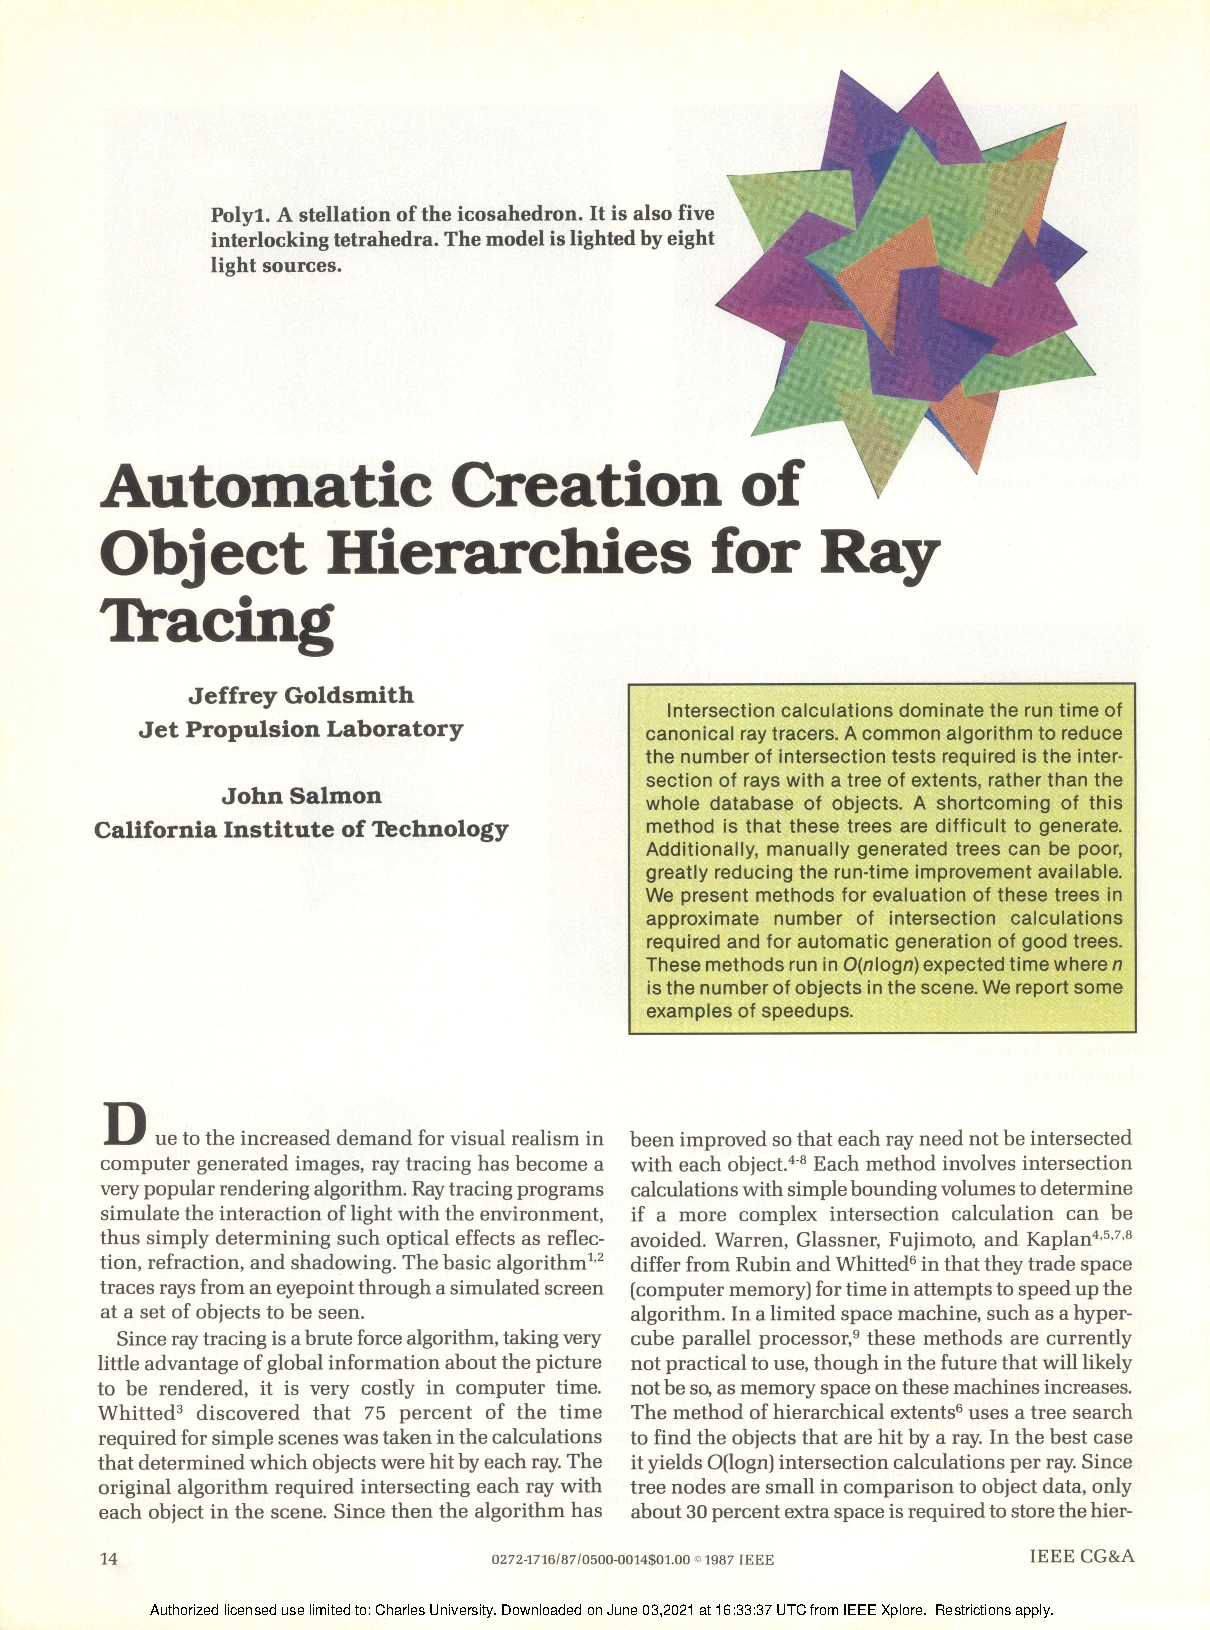
\includegraphics[width=.7\linewidth]{img/1 fundamentals/bvh.png}
	\caption{2D example of a bounding volume hierarchy, taken from \cite{pharr2016physically}. (a) represents the scene, consiting of simple shapes and their axis aligned bounding boxes and (b) the BVH tree structure associated with the scene from (a).}
	\label{fig:bvh}
\end{figure}

Bounding volumes should ideally be chosen, such that they fit the underlying geometry as close as possible in order to further reduce the number of unnecessary intersection test. However, a most commonly used volume is an \emph{axis aligned bounding box}, a hyperrectangle whose sides are parallel to the axis of the coordinate system. Such boxes might not enclose the geometry as tightly as possible, on the other side, testing for intersection becomes computationally cheap and not much memory is needed to store them.

These bounding volumes again can be enclosed in a bounding volume, and thus, complex hierarchies of bounding volumes can be formed.
A BVH then is a hierarchy of multiple of such bounding volumes, stored in a tree structure (commonly in binary trees). In the tree, the leafs represent the bounding boxes of the geometry primitives and the interior nodes are associated with bounding volumes enclosing the node's children. An example of such a tree structure is given by Figure \ref{fig:bvh}. The root of a BVH is typically a bounding box, enclosing the entire virtual scene.

Binary BVHs exhibit some convenient properties: \todo{fucking, check this dude! could be plain wrong} Every geometrical primitive is present in exactly one bounding box, and these bounding boxes do not overlap with each other. Thus, no primitive is possibly tested for intersection twice (unlike with KD trees, which are the subject of the next section). Furthermore, the amount of memory needed for storing a binary BVH is bounded. A BVH that is build over $n$ primitives obtains $2n-1$ total nodes, $n$ leave nodes and $n-1$ interior nodes \cite{pharr2016physically}. 

During ray tracing, the BVH is traversed and a cast ray is tested for intersection between a bounding box that is associated with the current tree node. If an intersection is found, the traversal continues in the node's children, otherwise traversing the sub tree rooted at that node is disregarded.

When compared to KD trees, BVHs usually require more time to be built, however, the ray-primitive-intersection testing is slightly faster. 

\subsection{KD Trees}

\begin{figure}
	\centering
	\includegraphics[width=1\linewidth]{img/1 fundamentals/kd_tree.png}
	\caption{Partition of a 2D scene in sub spaces A, B, C, and D with planes 0, 1, and 2. This figure is taken from \cite{hapala2011kd}.}
	\label{fig:kdtree}
\end{figure}

\emph{K-dimensional trees} (or KD trees), which were introduced by \cite{bentley1975multidimensional}, belong to the group of binary space partitioning trees (BSP trees). BSP trees recursively subdivide $k$ dimensional space with $k-1$ dimensional hyperplanes. One subdivision of space takes place when the number of geometric primitives contained in it are greater than a specified threshold. When one such subdivision happens, the space is divided into two smaller half-spaces for which this procedure is repeated until the number of primitives contained in a subdivided area is smaller or equal than the threshold. The hyperplanes that partition space are stored in a binary tree structure. The root of the tree is associated with the hyperplane splitting the bounding volume of the entire scene. Its children to the left are the hyperlanes and primitives in one half-plane that particular plane, and the children to the right are the planes and primitives that are located on the other one. The leaf nodes resemble a list of primitives being located in the area defined by their parent node's hyperplanes.

KD trees are a specialized case where the split-planes are perpendicular to one of the coordinate axis. During the recursive splitting, the axis to which the current plane is perpendicular to, is alternated. This allows for KD trees being efficiently constructed. However, \todo{check this too!} unlike with BVHs, primitives can be located in overlapping sub spaces, therefore intersection points may be calculated twice during ray tracing. 

When being compared to BVHs, the construction is faster (construction methods taking $O(n\log n)$ time exists \cite{wald2001interactive}.)

\section{Intel\textregistered's Embree Framework}
In spite the affect of various ray acceleration data structures and hardware optimizations, exploiting the full capabilities of modern CPUs, which exhibit different architectures and instruction sets and support different algorithms and data structures, remains challenging for ray tracing applications. 

Embree is a high performance rendering framework written in \texttt{C99} which addresses this problem. It offers a collection of vectorized kernels, being optimized for the communication with CPUs that support SSE, AVX, AVX2, AVX-512 and instruction sets. The provided kernels offer a variety of components, e.g. different types of BVHs, traversal algorithms and intersection algorithms, Figure \ref{fig:embree} provides an overview.
During a rendering process, Embree will decide on which components to use for building the acceleration structure and traversing it based information provided by the user and on the target CPU architecture. The later is performed by the "Ray Tracing Kernel Selection" layer of the hierarchy shown in Figure \ref{fig:embree}.

Interesting features of Embree are:
\begin{itemize}
	\setlength\itemsep{0.05em}
	\item 	Finding of the closest hit point, or alternatively any hit point,
	\item 	support for the cast of single rays, ray packets containing 4, 8 or 16 rays, and so-called ray streams of any desired number of rays,
	\item 	high-quality BVH builders,
	\item 	support for the Intel SPMD Program Compiler (ISPC) and the Intel Threading Building Blocks (TBB), and
	\item 	independence from any other graphics API such as OpenGL or DirectX
\end{itemize}

An API for the integration into existing rendering systems is provided and described in a detailed documentation \cite{embree2021Doc}. This documentation furthermore offers tutorial for the familiarization of the framework to new users. The name of the functions belonging to this API are preceded by the abbreviation \texttt{rtc} ("ray tracing kernels"), data types have the abbreviation \texttt{RTC} predeceasing their name. For example the variable \texttt{RTCScene} stores the virtual scene for Embree, and the function \texttt{rtcIntersect1()} performs the intersection testing with a single ray.

\begin{figure}
	\centering
	\includegraphics[width=1\linewidth]{img/1 fundamentals/embree_overview.png}
	\caption{System overview of Embree, taken from the SIGGRAPH presentation \citetitle{embreeSlides} \cite{embreeSlides}.}
	\label{fig:embree}
\end{figure}

Embree supports a variety of geometric shapes such as triangles, quads, and certain types of curves, such as Bézier curves, B-Splines and Catmull-Rom-Splines.
Another notable feature of Embree is the support of custom geometries. These will be referred to as \emph{User defined geometries}. 

Embree is open source, and therefore publicly available. Supported platforms are (32-bit and 64-bit), Linux (64-bit), and macOS (64-bit). The latest version of Embree at the time of writing this thesis is 3.13.0. 

\subsubsection{Ray Tracing in Embree}
Embree follows a device concept, allowing for the use of the Embree API by different components of the image synthesis application without interfering each other. An \texttt{RTCDevice} can be created with the function \texttt{rtcNewDevice} and released via the function \texttt{rtcReleaseDevice}. Such device types are used by Embree to create further components, such as virtual scenes which serve as the container for various scene geometry. A scene in Embree, represented by the data type \texttt{RTCScene}, can be created via the function \texttt{rtcNewScene}, to which the \texttt{RTCDevice} is passed to as an argument, and released via the function \texttt{rtcReleaseScene}. Different geometries can be attached or detached by the functions \texttt{rtcAttachGeometry}, which will furthermore assign a unique ID to the geometry, and \texttt{rtcDetachGeometry}. Once an \texttt{RTCGeometry} is attached to the \texttt{RTCScene}, it can be released via the call of the function \texttt{rtcReleaseGeometry}.
After the attachment of the complete scene geometry, the scene can be committed by calling the function \texttt{rtcCommitScene} in order to trigger the creation of Embree's internal acceleration structures. After the invocation of this function, the individual geometries cannot be edited or manipulated.

Geometries in Embree are represented by a \texttt{RTCGeometry} data type. These types can be created with the function \texttt{rtcNewGeometry} which takes the \texttt{RTCDevice} and an enum specifying the geometry type (e.g. triangle, quad, user defined geometry) as input parameters. In case the geometry being a triangle, quadrangle or a type of curve, so-called \emph{geometry buffers} can be created and linked to the \texttt{RTCGeometry} by invoking the function \texttt{rtcSetNewGeometryBuffer}. These buffers will store information such as vertices, indices and surface normals of the geometry.  

In order to initialize a user defined geometry, one has to provide a function for calculating the bounding box for the geometry, a function for intersection testing and another function for occlusion testings. These functions are passed to Embree as callback functions. Furthermore, the number of geometric primitives, which together compose the geometry, has to be set, and a so-called \emph{User data pointer} associated with the geometry. A user data pointer points to the representation of the geometry by the rendering application in memory. In the interior of the callback function for calculating the intersection with the user defined geometry, the original representation of the geometry can be easily retrieved via this pointer. The passing of the various callback functions to Embree is done via invocation of the functions \texttt{rtcSetGeometryUserPrimitiveCount}, \texttt{rtcSetGeometryUserData}, \texttt{rtcSetGeometryBoundsFunction}, \texttt{rtcSetGeometryIntersectFunction}, \newline and \texttt{rtcSetGeometryOccludedFunction}.

Once the \texttt{RTCDevice} and the \texttt{RTCScene} are set up, the scene geometry is attached to the \texttt{RTCScene}, and the internal acceleration data structures have been built, nothing stands in the way of performing the actual ray tracing with Embree. 

In the following example, only ray tracing with single rays as opposed to packet ray tracing is considered. We will furthermore not consider instancing, due to the reason that this feature does not find use in the work of this thesis.

In order to ray trace a virtual scene, a per ray query intersection context, \texttt{RTCIntersectContext}, has to be set up via the function \texttt{rtcInitIntersectContext}. This structure is used for the configuration of intersection flags, among other things. 
Subsequently, a \texttt{RTCRayHit} struct is declared. This struct is composed of an \texttt{RTCRay} struct, abstracting the ray that is used by Embree to preform the intersection testing, and an \texttt{RTCHit} struct, in which information concerning the intersection point, such as the surface normal, the barycentric UV coordinates of the point, and the geometry ID associated with the intersected geometry are stored.
The \texttt{RTCRay} struct stores the ray orientation and direction, so-called \texttt{tnear} and \texttt{tfar} values, indicating the boundaries of a range of possible hit distances, and other information such as an id for the ray, a ray mask and a \texttt{time} value useful when motion blur is desired.
When the target ray tracing application is generating a ray, the values of the \texttt{RTCRay} struct are updated with the ray orientation and direction. The \texttt{tnear} value is usually set to zero and the \texttt{tfar} value is set to infinity. The geometry ID of the \texttt{RTCHit} struct is initialized with the macro \texttt{RTC\_INVALID\_GEOMETRY\_ID}.

After the \texttt{RTCIntersectContext} and the \texttt{RTCRayHit} structs have been successfully initialized and updated, the ray-primitive intersection testing is performed via invocation of the function \texttt{rtcIntersect1} to which the \texttt{RTCScene}, a reference to both the \texttt{RTCIntersectContext} and the \texttt{RTCRayHit} are passed as arguments. In case of a found intersection, this function will update the \texttt{tfar} value of the \texttt{RTCRay} with the closest hit distance and the geometry ID of the \texttt{RTCHit} with the geometry ID associated to the intersected geometry.

In case of performing intersection testing between a user defined geometry and a ray, these values have to be updated manually inside the intersection function that was passed to Embree as a callback function.

When the intersecting testing procedure has finished, the geometry ID of the \texttt{RTCHit} will give insight on whether an intersection was found or not. If the value of this variable remains \texttt{RTC\_INVALID\_GEOMETRY\_ID}, one can conclude that no intersection was found. Otherwise, an intersection was found and the \texttt{RTCRay} and \texttt{RTCHit} components of the \texttt{RTCRayHit} will provide the hit distance, the coordinates of the surface normal at the intersection point and the UV coordinates of the intersection point.